%%%%%%%%%%%%%%%%%%%%%%%%%%%%%%%%%%%%%%%%%%%%
%% CASPER STEINMANNS KU-GREEN BEAMER HEADER
%%%%%%%%%%%%%%%%%%%%%%%%%%%%%%%%%%%%%%%%%%%%

\documentclass{beamer}
\usepackage{pgf}
\usepackage{beamerthemesplit}
\usepackage{listings}
\usepackage{booktabs}

\definecolor{kugreen}{RGB}{50,93,61}
\definecolor{kugreenlys}{RGB}{132,158,139}
\definecolor{kugreenlyslys}{RGB}{173,190,177}
\definecolor{kugreenlyslyslys}{RGB}{214,223,216}

\setbeamercovered{transparent}
\usetheme[compress,height=8mm]{Rochester}
\usecolortheme[named=kugreen]{structure}

\usepackage{amsmath}
\usepackage[T1]{fontenc}
%\usepackage[latin1]{inputenc}
\usepackage[utf8]{inputenc}

\newcommand{\chem}[1]   {\ensuremath{\mathrm{#1}}}
\newcommand{\Rm}[1]     {\mathrm{#1}}
\newcommand{\unit}[1]   {\,\mathrm{#1}}
\newcommand{\htoon}[1]  {\chem{(H_2O)_{#1}}}

% JCK
\renewcommand{\vec}[1]{{\bf #1}} % Lars likes this better than arrow

\beamertemplatenavigationsymbolsempty % Removes the navigation bar
\setbeamertemplate{footline}{}

% TITLE AND OTHER STUFF GOES HERE
\title[University of Copenhagen]{Molekylær Statistik, Eksamens Projekter}
\author{
  Anders S. Christensen \newline andersx@nano.ku.dk \newline
  \newline
  Jimmy C. Kromann \newline jimmy@charnley.dk
}
\institute{Kemisk Institut \\ Københavns Universitet}

% NOW THE DOCUMENT BEGINS
\begin{document}

\lstset{
language=Python,                        % Code langugage
%commentstyle=\color{gray},              % Comments font
%basicstyle=\small,                      % Code font, Examples: \footnotesize, \ttfamily
numbers=left,                           % Line nums position
numberstyle=\tiny,                      % Line-numbers fonts
stepnumber=1,                           % Step between two line-numbers
numbersep=5pt,                          % How far are line-numbers from code
frame=none,                             % A frame around the code
tabsize=4,                              % Default tab size
captionpos=b,                           % Caption-position = bottom
breaklines=true,                        % Automatic line breaking?
breakatwhitespace=false,                % Automatic breaks only at whitespace?
showspaces=false,                       % Dont make spaces visible
showtabs=false,                         % Dont make tabls visible
keywordstyle=\color{blue},
stringstyle=\color{red},
commentstyle=\color{green},
morecomment=[l][\color{magenta}]{\#}
}


\frame{\titlepage \vspace{-0.5cm}}


% ***************************************************
% BEGIN FRAMES
% ***************************************************

\frame
{
    \frametitle{Projekter}

    \begin{enumerate}
      \item Diffusion Coefficient of the Lennard-Jones Fluid
      \item Genetic Algorithm
      \item Ising Spin-Lattice Model
    \end{enumerate}
}

\frame
{
    \frametitle{Projekt 1: Diffusion}

}


\frame
{
    \frametitle{Projekt 2: Genetic}

}


\frame{ %MY BRACKET STYLE IS AWESUM!
    \frametitle{Projekt 3: 2D Ising Model}
    %\frametitle{Projekt 3: JYMMMY ER LOLAWL}


    \textbf{Representation of 2D magnetic solid}

    \begin{columns}[c]
        \column{2.0in}
            \begin{itemize}

                \item Monte Carlo is used to simulate fluctuations
                \vspace{0.2in}

            \uncover<2->{

                \item $ \epsilon_{ij} = -J \cdot S_i \cdot S_j$
                \vspace{0.2in}
            }

            \uncover<3->{
                \item Boltzmann Distribution:\\
                \vspace{0.1in}
                     $p(E_i) \propto \exp \left( \frac{-E_i}{k_{\mathrm{B}}T} \right)$
            }

            \end{itemize}

        \column{2.0in}
            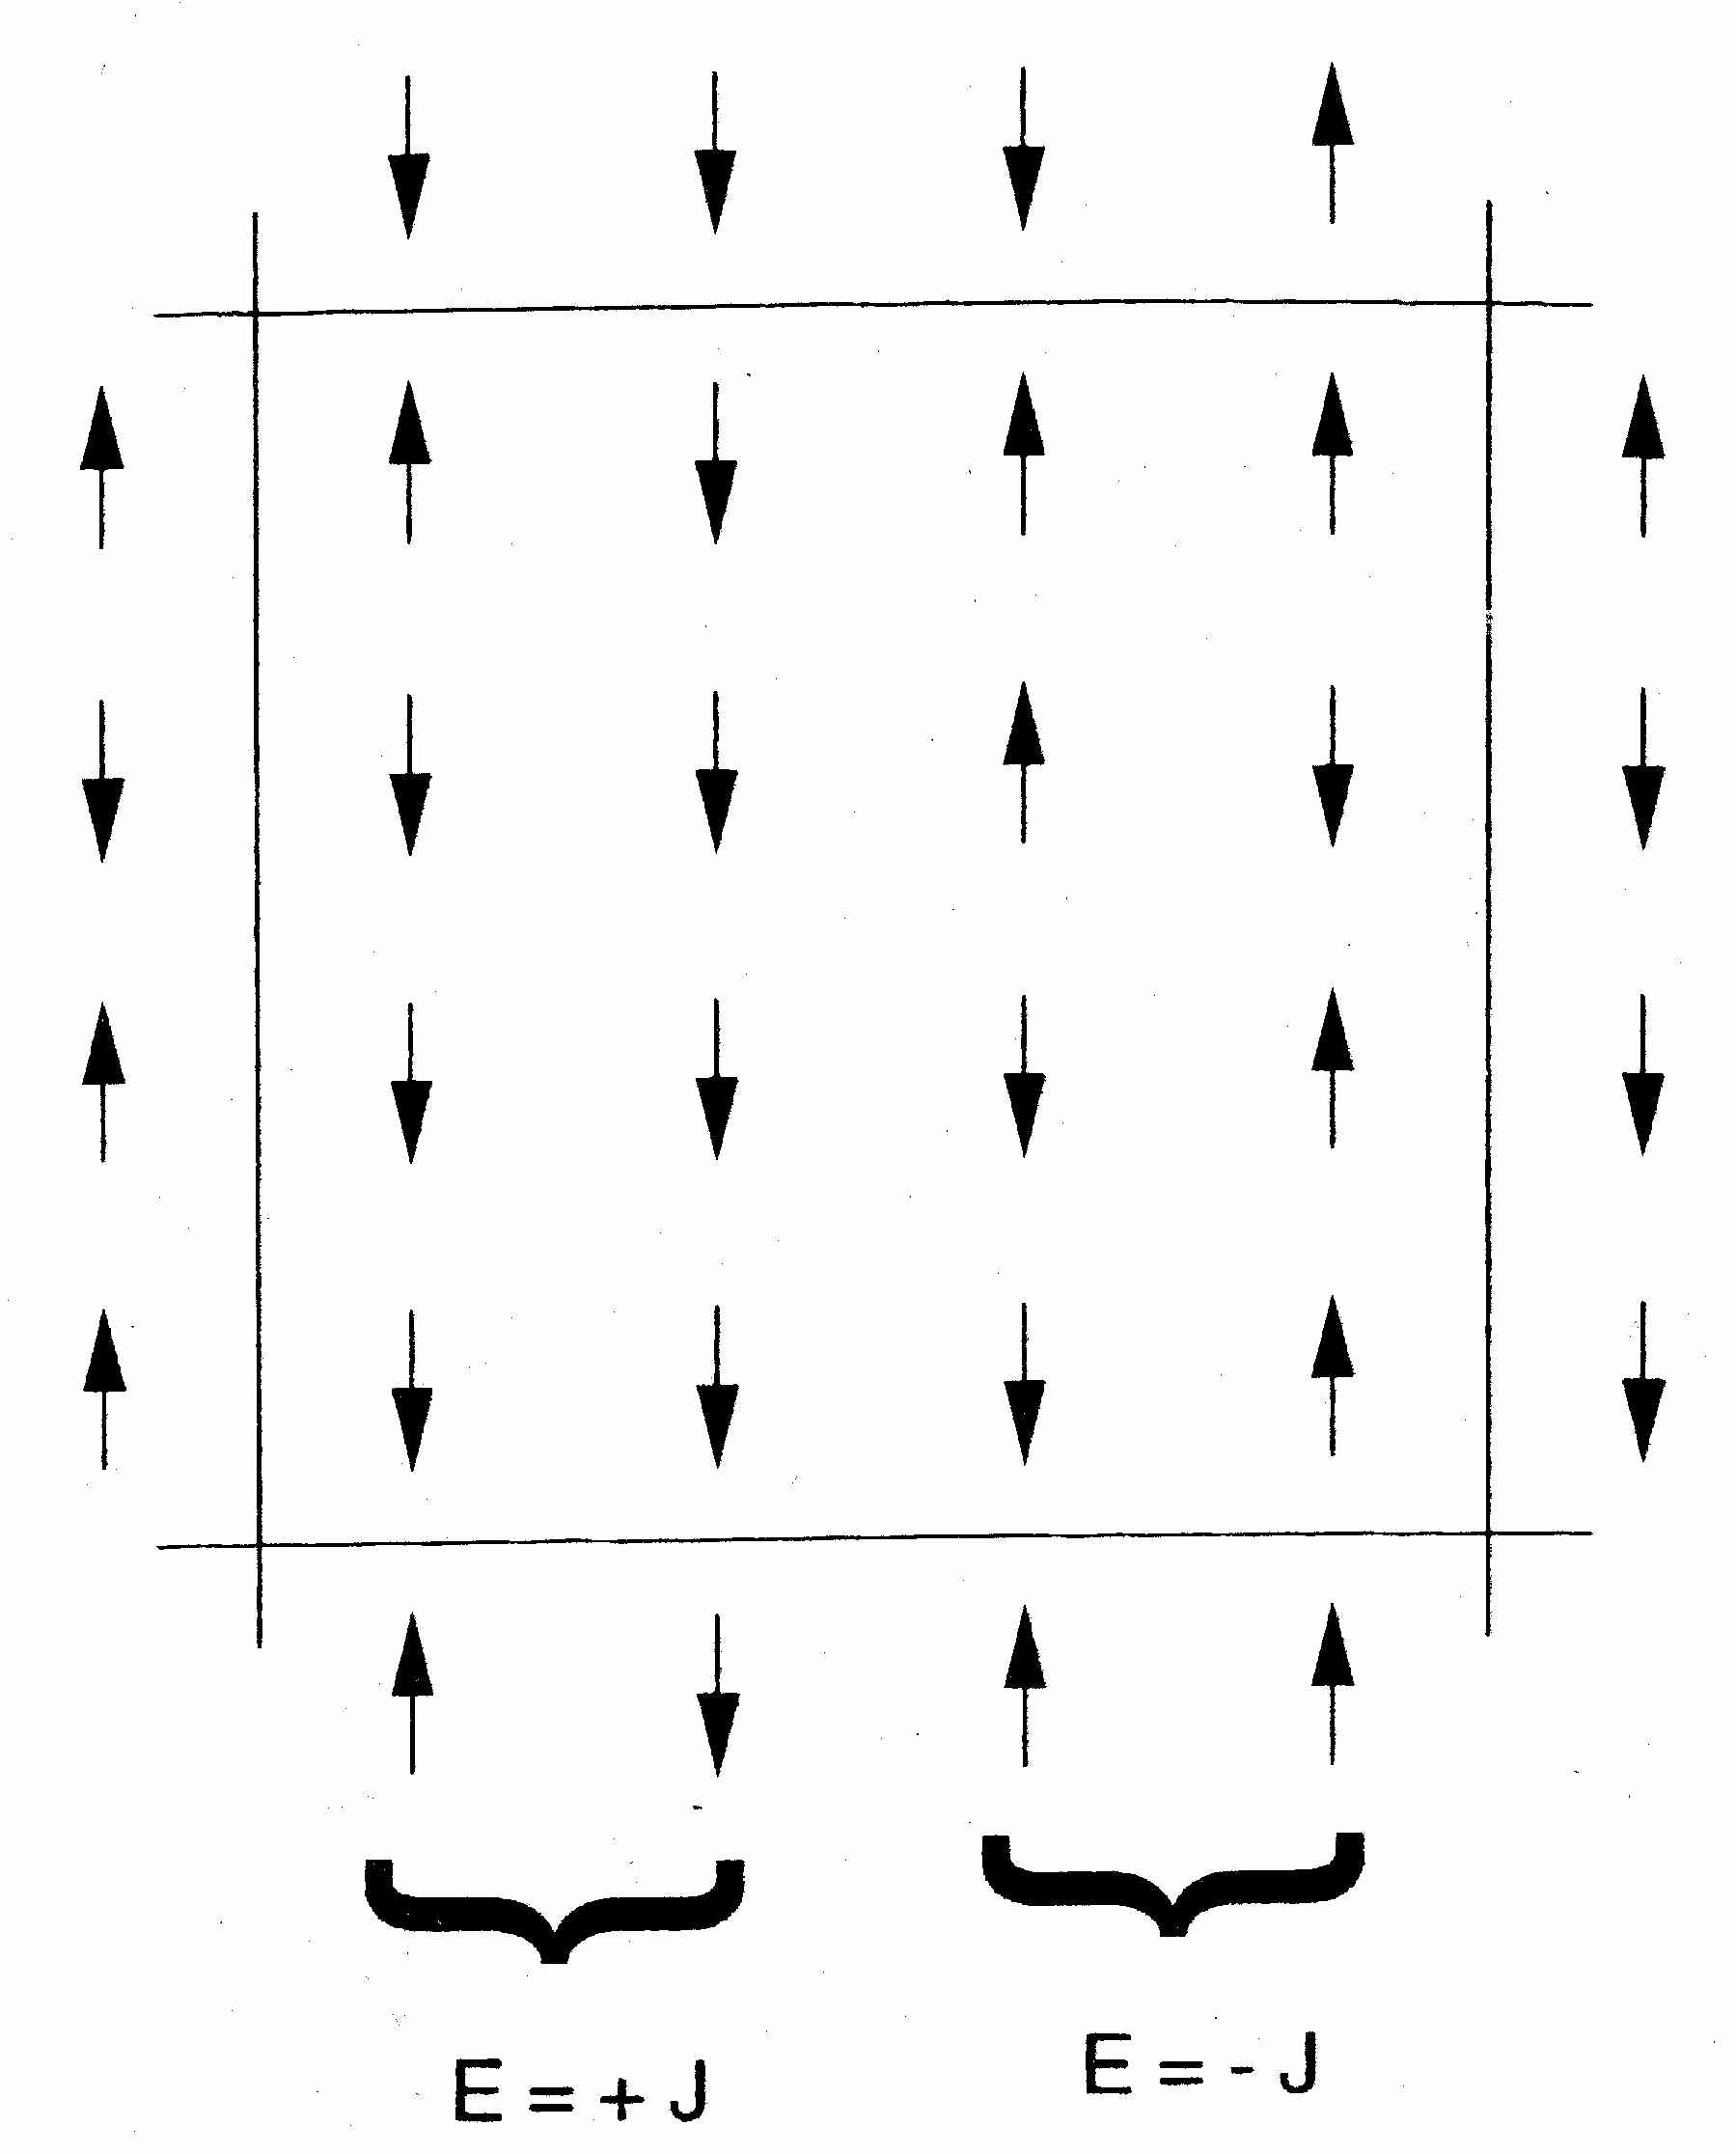
\includegraphics[width=2in]{lattice.jpg}


    \end{columns}

}



\frame{ %MY BRACKET STYLE IS AWESUM!
    \frametitle{Projekt 3: 2D Ising Model}

    \textbf{Phase transitions:} High $\rightarrow$ low temperature\\
    \vspace{0.1in}
    \begin{columns}[c]
    \column{2.5in}
        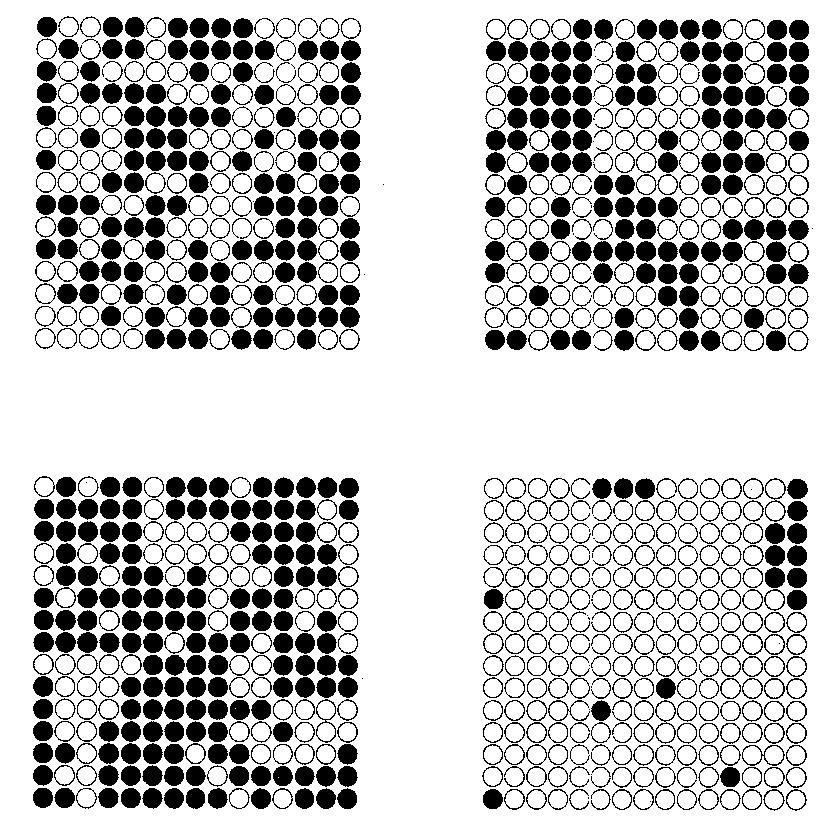
\includegraphics[width=2.5in]{temperatures.jpg}
    \column{2.0in}
        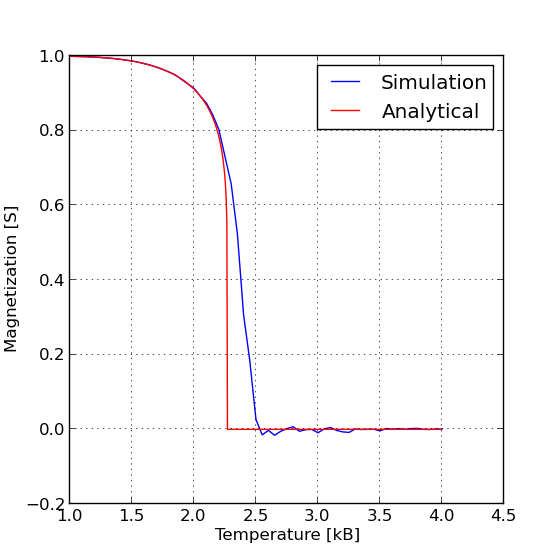
\includegraphics[width=2in]{mag_anal.png}
    \end{columns}

}



\frame{%MY BRACKET STYLE IS AWESUM!
    \frametitle{Projekt 3: 2D Ising Model}

    \textbf{Project description:}\\

    \begin{itemize}

        \item Implement the Monte Carlo Metropolis-Hastings algorithm in
              Python (with Numpy).

    \vspace{0.1in}
        \uncover<2->{
            \item Simulate the 2D Ising spin lattice.
        }
    
    \vspace{0.1in}
        \uncover<3->{
            \item Calculate interesting properties such as heat capacity, magnetization, and
              magnetic susceptibility.
        }
    \end{itemize}

%    \begin{center}
%       \phantom{\includegraphics<-3>[width=1.5in]{rageface1.png}}
%       \includegraphics<4->[width=1.54in]{rageface1.png}
%    \end{center}
}




\frame{%MY BRACKET STYLE IS BESTBESTBEST!!!!!!!!!!!!!!!!!!!!!!!!!!!!!!!!!!!!!!!!!!!!!!!!!!!!!!!!!!!!!!!!!!!!!!!!!!!!!!!!!!!
%\frame{%MY BRACKET STYLE IS BESTBESTBEST!!!!!!!!!!!!!!!!!!!!!!!!!!!!!!!!!!!!!!!!!!!!!!!!!!!!!!!!!!!!!!!!!!!!!!!!!!!!!!!!!!!
%\frame{%MY BRACKET STYLE IS BESTBESTBEST!!!!!!!!!!!!!!!!!!!!!!!!!!!!!!!!!!!!!!!!!!!!!!!!!!!!!!!!!!!!!!!!!!!!!!!!!!!!!!!!!!!
%\frame{%MY BRACKET STYLE IS BESTBESTBEST!!!!!!!!!!!!!!!!!!!!!!!!!!!!!!!!!!!!!!!!!!!!!!!!!!!!!!!!!!!!!!!!!!!!!!!!!!!!!!!!!!!
%\frame{%MY BRACKET STYLE IS BESTBESTBEST!!!!!!!!!!!!!!!!!!!!!!!!!!!!!!!!!!!!!!!!!!!!!!!!!!!!!!!!!!!!!!!!!!!!!!!!!!!!!!!!!!!
    \frametitle{Projekskrivning}


    \textbf{Generelt:}

    \begin{itemize}
        \item Programmeringen udføres i små grupper. 
        \item Rapporterne er individuelle.

    \end{itemize}
    \vspace{0.2in}
    \uncover<2->{

    \textbf{Vejledere:}

    \begin{itemize}

        \item Jimmy er vejleder på diffusion og genetisk algoritme.

        \item Anders er vejleder på Ising-modellen.

    \end{itemize}

    }
    
    \uncover<3->{

    \vspace{0.2in}

    \textbf{Hvis I sidder fast:}

    }
    \begin{enumerate}

        \uncover<4->{
            \item Arbejd sammen med en anden gruppe.
        }

        \uncover<5->{
            \item Skriv en mail og aftal at mødes med vejlederen.
        }
    \end{enumerate}


}










% ***************************************************
% END FRAMES
% ***************************************************

\end{document}

